\subsubsection{Supernova Neutrinos}

\paragraph{Motivation}

The neutrino burst detected from the next galactic Supernova will provide us with a wealth of information on the dynamics of the core collapse (neutronization, reheating, proto-neutron star cooling) and the properties of the neutrinos themselves (mass hierarchy, absolute mass scale, collective oscillations). Since the first detection of Supernova neutrinos in 1987, the scientific community has not become tired to predict new effects and their signatures that are potentially to be extracted from the neutrino signal. So while we are uncertain what to expect from the next event and how different effects will overlay, it is beyond doubt that only a concerted effort making use of the complementary strengths of all the neutrino observatories available will enable us to extract the full amount of information. Moreover, this combined analysis has to reach beyond neutrino detectors, including gravitational wave and (if present) optical signatures to appreciate the full picture.

If a Supernova neutrino burst would pass by the Earth today, hundreds of events would be expected in several smaller observatories (LVD, Borexino, KamLAND, SNO+, HALO to name but a few). However, the largest event statistics would be collected by the two large Cherenkov detectors, Super-Kamiokande (SK) and IceCube. Ten years from now, we may expect that two further players will appear on the stage: JUNO offering a liquid scintillator target, and DUNE allowing SN neutrino detection in liquid argon. In the most simplified picture, SK, JUNO and IceCube will dominate the information on $\bar\nu_e$ flux and energies, while DUNE has the potential for a high-statistics $\nu_e$ measurement. JUNO will provide information on the combined flux of $\nu_\mu$ and $\nu_\tau$ and antineutrinos (in the following, we use the conventional denotation $\nu_x$).

\paragraph{Impact of THEIA} In the following, we assume the THEIA-ii detector configuration, i.e.~a 50\,kt neutrino target filled with a WbLS containing 10\,\% of organic scintillator. With 90\,\% optical coverage, the expected photoelectron yield for a 10\,\%-WbLS is $\sim$200\,p.e./MeV (75\,\% scintillation), providing a stochastic energy resolution of 7\,\%. Thus, THEIA will provide a threshold in the low MeV range and $-$ given the high coverage $-$ spectroscopic capabilities close to that of current-day organic liquid scintillator detectors. Importantly, THEIA will provide a clear neutron tag, allowing to discriminate Inverse Beta Decay (IBD) events from other single-event backgrounds.
\medskip\\
Given this additional features, what can THEIA add to the global picture of SN neutrino observations? 
\begin{itemize}
\item a high-statistics IBD ($\bar\nu_e$ ) signal, offering considerably better energy resolution than SK and about twice its statistics; both will prove very useful when trying to correlate spectral features changing over time with other signals, e.g.~gravitational wave emission during the SASI phase, or when looking for energy-dependent oscillation patterns (e.g.~the spectral swaps induced by collective oscillations)
\item improved pointing accuracy for the $\nu_e$ elastic scattering signal, improving the current day $\sim$3$^\circ$ resolution of SK to the level of 1$^\circ$ or better. The key is the almost complete event-by-event subtraction of IBD events enabled by the neutron capture tag \cite{Tomas:2003xn}; SK+Gd can expect a similar improvement but offers a neutron tagging efficiency of only $\sim$70\,\%
\item the chance to glimpse the initial $\nu_e$ neutronization burst \cite{Kachelriess:2004ds}: however, as $\cal O$(10) events are expected for a SN at 10\,kpc, detailed information can only be expected for a relatively nearby Supernova
\item relative to SK and JUNO, a $\bar\nu_e$ detector on the other side of the Earth, allowing to study Earth matter effects in $\bar\nu_e$ in a direct spectral comparison; note that, again, energy resolution is a key parameter here.
\end{itemize}

\paragraph{Spectroscopy of SN neutrinos in THEIA}

Compared to all other running and upcoming detectors (except Hyper-Kamiokande), 50\,kt of WbLS will constitute the largest neutrino target, roughly doubling the available statistics of IBDs in water (SK) and scintillator (JUNO) detectors. Moreover, THEIA will provide both good energy and directional resolution, offering handles to discriminate between different neutrino reaction channels.

As stated above, present knowledge of the SN neutrino emission and neutrino properties does not allow for a precise prediction of the expected signal. Nevertheless, to provide a scale of the expected signal we list in table \ref{tab:snrates} the time-integrated event rates for a Supernova in 10\,kpc distance (close to the galactic center), using energies and fluxes predicted by the GVKM (Gava-Kneller-Volpe-McLaughlin) model \cite{Gava:2009pj} and the cross-sections provided by the SNOwGLoBES framework.

\begin{table}[h!]
\centering
\begin{tabular}{lclr}
\hline
Channel & & Reaction & Event rate \\
\hline
Inverse Beta Decay & (IBD) & $\bar\nu_e+p\to n+e^+$ & 9,900 \\
 Electron Scattering & (ES) &$\nu+e \to e+\nu$ & 480 \\
 CC on $^{16}$O & ($\bar\nu_e$O) & $\nu_e+ {^{16}{\rm O}} \to  {^{16}{\rm F}}+e^-$ & 170 \\
 & ($\nu_e$O) & $\bar\nu_e+ {^{16}{\rm O}} \to  {^{16}{\rm N}}+e^+$ & 220 \\
NC on $^{16}$O & (NC) &  $\nu + {^{16}{\rm O}} \to  {^{16}{\rm O}^*}+\nu$ & 550 \\
\hline
\end{tabular}
\caption{Neutrino event rates expected in 50\,kt of WbLS (10\,\% scintillator) for a core-collapse Supernova at 10\,kpc distance. Neutrino spectra and fluxes follow the GVKM model \cite{Gava:2009pj}.}
\label{tab:snrates}
\end{table}

\noindent {\bf Event rates.} The signal is vastly dominated by the $\bar\nu_e$-induced IBD events, followed by the NC reactions of all neutrino flavors on oxygen and elastic scattering off electrons. Note that as WbLS contains as well carbohydrates, THEIA will detect relevant numbers of neutrino events on carbon: For a 10\,\% WbLS, $\sim$250 events from NC carbon reactions are expected, inducing a gamma peak at 15\,MeV (not shown in fig.~\ref{fig:snspectra}), adding to the information on the integrated neutrino flux.
\medskip\\
{\bf Energy spectrum} Given its large target mass and good energy resolution, THEIA will offer detailed spectral information for the $\bar\nu_e$ flux (based on IBD events). Moreover, less precise but still relevant spectral data will be available for all other neutrino flavors that are detected in their hundreds. In figure \ref{fig:snspectra}, we show the expected event spectra as a function of their visible energy, already smeared with a 7\,\% energy resolution. As for the rate, the IBD signal dominates the interaction rates for all energies, with the noteworthy exception of the two low-energy $\gamma$ lines from the NC reaction on oxygen. However, differently from current-day water Cherenkov detectors, the neutron tag for IBD events allows to subtract the IBD signal on an event-by-event basis, providing better access for a separate study of the subdominant reaction channels. As a consequence, the gamma lines from the NC reaction are easy to extract from the remaining spectrum, providing a flavor-independent measurement of the neutrino flux \cite{Langanke:1995he,Haxton:1987kc}. Moreover, the presence of scintillation light and high energy resolution enables separate detection of the strongest gamma lines and thus a measurement of their relative spectral contributions. In case of a very efficient IBD subtraction (close to 100\,\% efficiency), there will be even some potential to separate the remaining ES, $\nu_e$O and $\bar\nu_e$O channels: ES events are strongly correlated with the SN direction and will stand out in any case (see below). Moreover, the re-decay of $^{16}$N potentially offers a delayed coincidence signature for $\bar\nu_e$O events: The remaining $\nu_e$O would then provide access to a small but pure sample of electron neutrino events. 
\begin{figure}[h!]
\centering
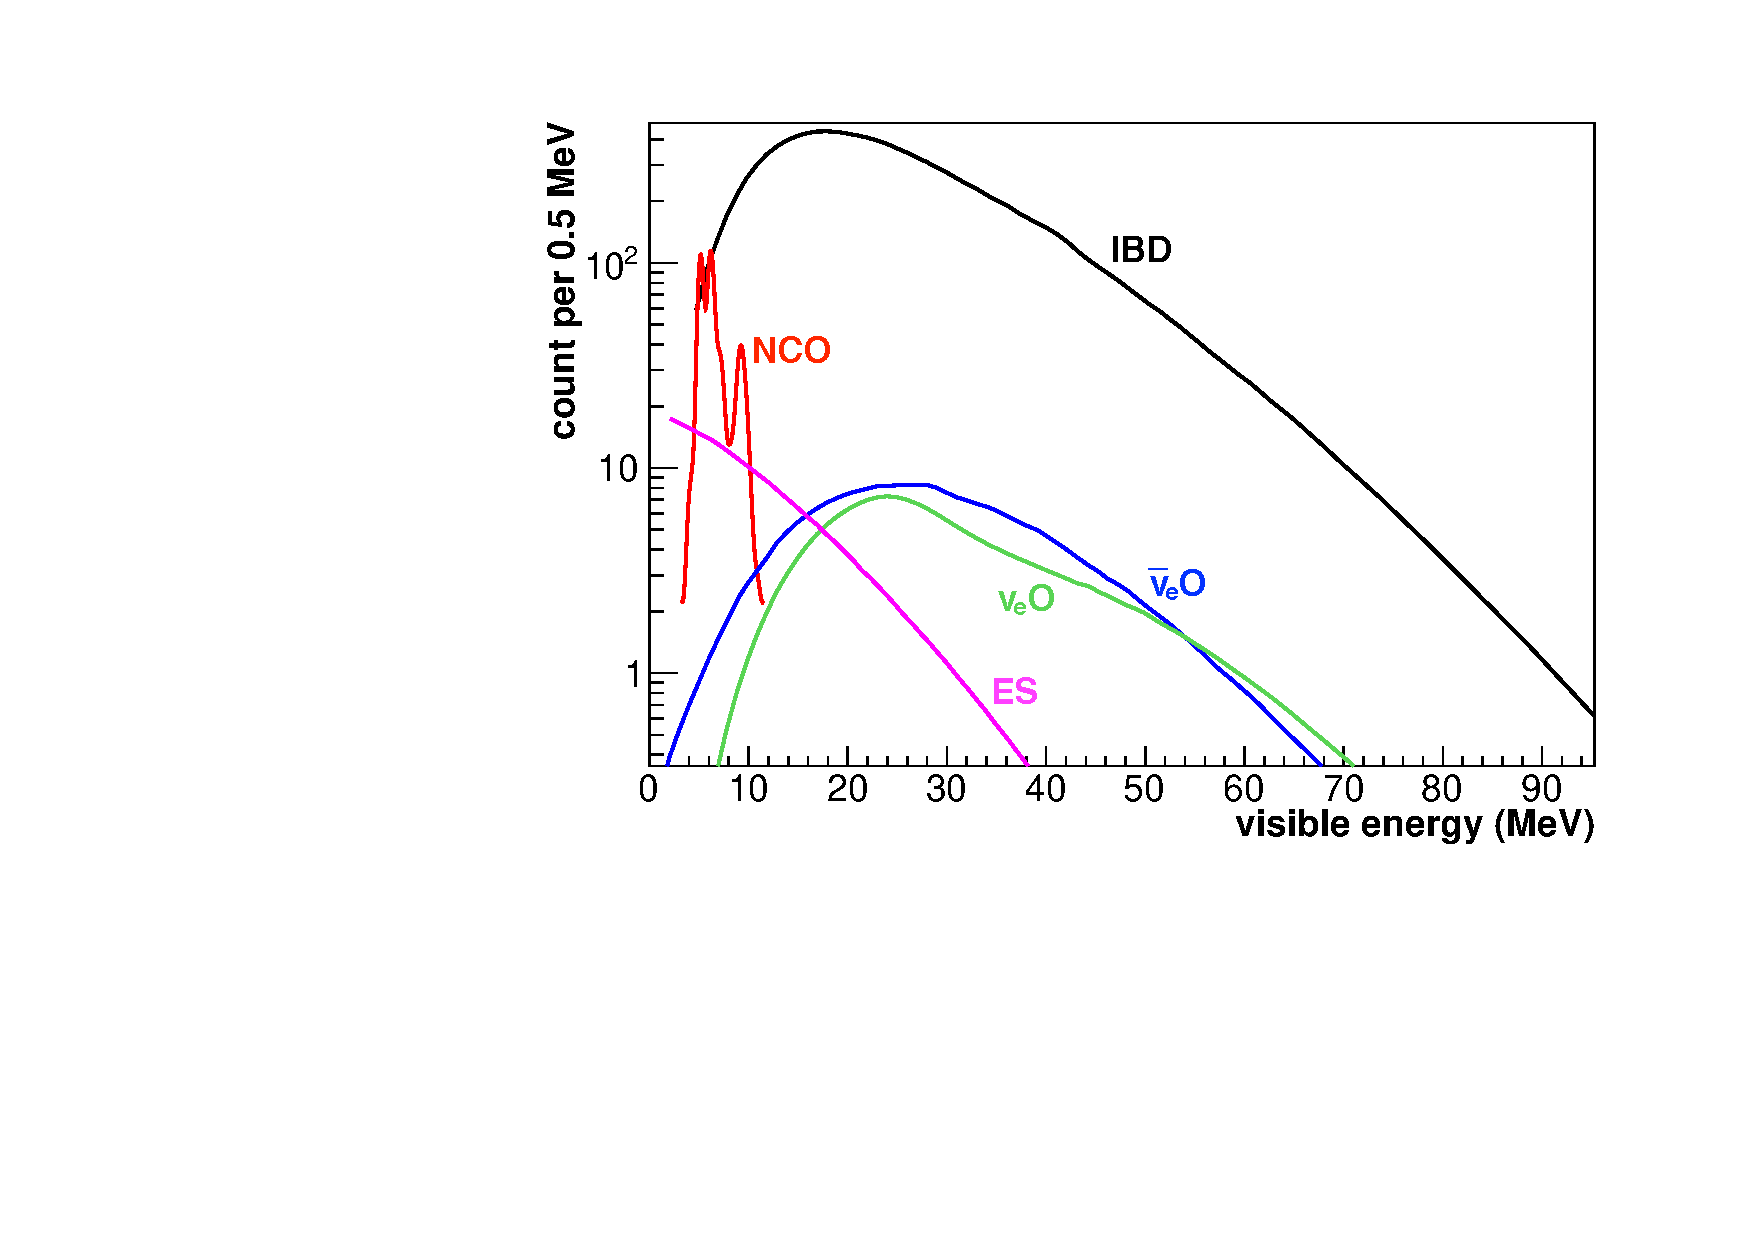
\includegraphics[width=0.67\textwidth]{sn_spectra.pdf}
\caption{Visible energy spectra for prompt events expected in 50\,kt of WbLS, assuming a Gaussian energy resolution of 7\,\% at 1\,MeV. Neutrino spectra and fluxes follow the GVKM model \cite{Gava:2009pj}.}
\label{fig:snspectra}
\end{figure}
\medskip\\
\noindent{\bf Time-dependent features} A time-dependent measurement of the neutrino signal is especially interesting for studying the different phases and physical processes underlying the core collapse. For a Supernova in 10\,kpc distance, the initial neutronization burst will translate only to a small number of ES and $\nu_e$O events in THEIA, $\cal O$(10). However, if the SN were to happen closer and if the information of several detectors (especially DUNE) is combined, energy, flux and flavor content may be studied in detail. On its own, THEIA will provide detailed spectral information of the $\bar\nu_e$ flux during the accretion phase, nicely complementing the flux information available from IceCube. 
\medskip\\
{\bf SN neutrino pointing.} In Water Cherenkov Detectors like SK, the direction of the incoming neutrino burst can be determined based on the recoil electrons from ES: Given the relatively large neutrino energies, the electrons are very tightly aligned with the initial momentum of the neutrino. In SK, this will be sufficient to pinpoint the location of the SN within 3-4 degrees \cite{Abe:2016waf}. The most important factor limiting resolution in this case is the relatively high background formed by the only slightly directional positrons from IBD interactions. In the angular distribution of events, a peak consisting of $\sim10^2$ ES events has to be found over a flat background of several thousand IBDs.

It has been suggested (e.g.~in \cite{Tomas:2003xn}) that the directional resolution can be considerably enhanced if the IBD events can be discriminated based on the delayed neutron tag, reducing the flat background. This represents one of the key features of SN neutrino detection in THEIA: As an example, the left panel in figure~\ref{fig:snpointing} shows the angular distribution for an SN neutrino burst (Wilson model \cite{Totani:1997vj}, 10\,kpc distance), where an efficiency of 90\,\% is assumed for IBD rejection: While the ES events are clearly peaked in the direction of the SN ($\Delta\theta=\Delta\phi=0^\circ$), the reduced IBD background constitutes only a minor background noise. 

We studied the effect of IBD background reduction on the directional resolution based on a toy MC of the signal. For this, we fitted the output angular distribution with a radial exponential plus flat background resolution, regarding three different cases: No, 90\,\% and full IBD reduction with full detection efficiency for ES events. For the latter, we considered full event kinematics (linking electron and neutrino momentum directions) and an intrinsic angular resolution of 10$^\circ$. The results are depicted in the right panel of figure~\ref{fig:snpointing}, once for a fiducial mass of 45\,kt in the THEIA-ii configuration where close to full detection efficiency for the delayed neutron tag can be assumed, and once for half this  mass to allow for an easier comparison to current SK pointing capabilities. While we can reproduce the $\cal O$(3-4$^\circ$) pointing accuracy of SK, THEIA will reach an angular resolution of close to 1$^{\circ}$.

It should be noted that SK+Gd will feature as well improved pointing precision based on the available delayed neutron tag. For this case, angular resolution can be estimated to $\sim$2$^{\circ}$.
\begin{figure}[h!]
\centering
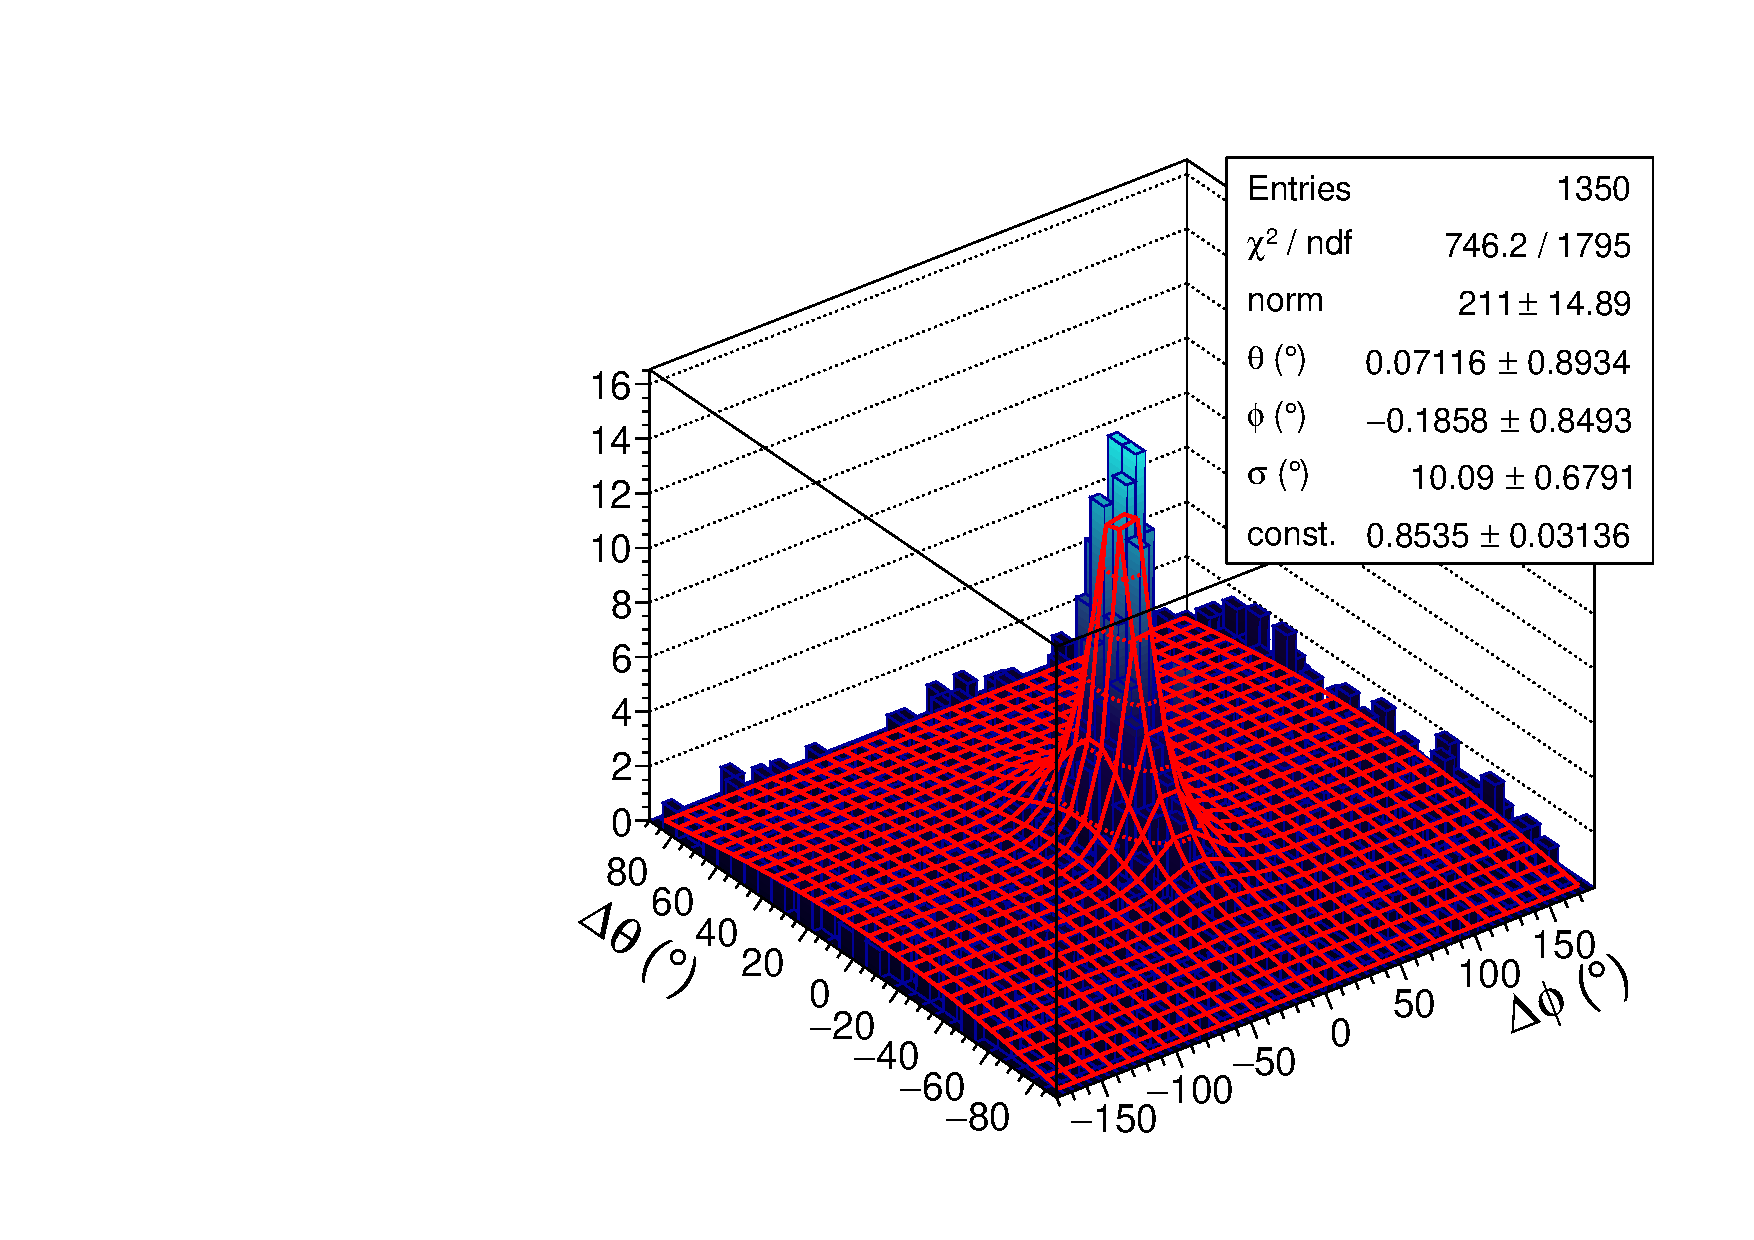
\includegraphics[width=0.5\textwidth]{sn_directionality_fit.pdf}
\hfill
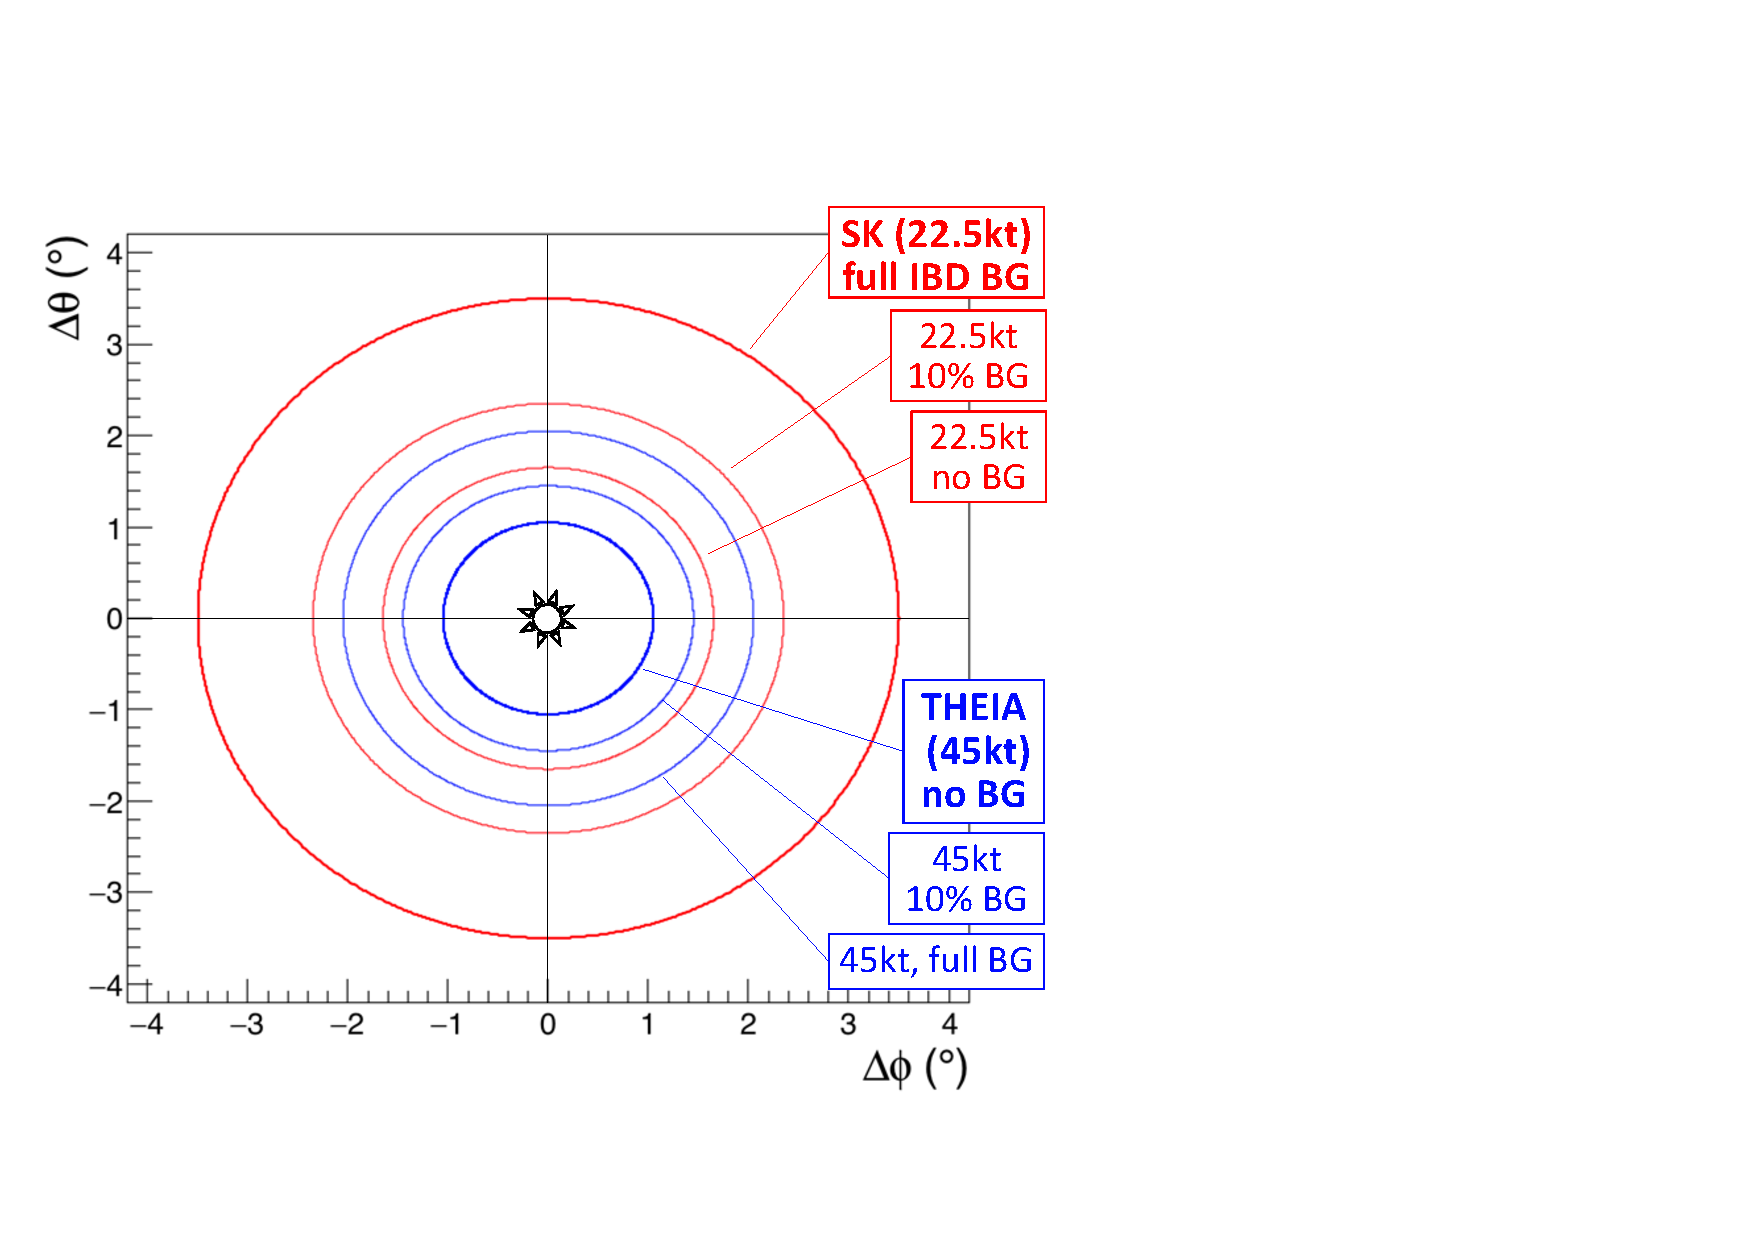
\includegraphics[width=0.46\textwidth]{sn_position_resolution.pdf}
\caption{SN pointing capability of THEIA, based on the reconstruction of the ES directional signal. {\it Left panel:} Example angular distribution, assuming 90\,\% in the flat IBD spectrum. Based on a fit to this and similar distributions (red net), the {\it right panel} depicts the pointing accuracy for THEIA, assuming different IBD background levels for 45\,kt as well as 22.5\,kt target mass.}
\label{fig:snpointing}
\end{figure}
